\documentclass{beamer}
%
% Choose how your presentation looks.
%
% For more themes, color themes and font themes, see:
% http://deic.uab.es/~iblanes/beamer_gallery/index_by_theme.html
%
\mode<presentation>
{
  \usetheme{default}      % or try Darmstadt, Madrid, Warsaw, ...
  \usecolortheme{default} % or try albatross, beaver, crane, ...
  \usefonttheme{default}  % or try serif, structurebold, ...
  \setbeamertemplate{navigation symbols}{}
  \setbeamertemplate{caption}[numbered]
} 

\usepackage[english]{babel}
\usepackage[utf8]{inputenc}
\usepackage[T1]{fontenc}

\title[Your Short Title]{Control Systems}
\author{Neil {EE18BTECH11031}}
\institute{IIT Hyderabad}
\date{12th January, 2020}

\begin{document}

\begin{frame}
  \titlepage
\end{frame}

% Uncomment these lines for an automatically generated outline.
%\begin{frame}{Outline}
%  \tableofcontents
%\end{frame}

\section{Question}

\begin{frame}{Question}

\begin{block}{GATE 2017; \\Q47}
A second-order LTI system is described by the following state equations: 
\begin{Large}
\begin{itemize}
    \item $\frac{\partial x_1(t)}{\partial t} - x_2(t) = 0$
    \item $\frac{\partial x_2(t)}{\partial t} + 2x_1(t) + 3x_2(t) = r(t)$
\end{itemize}
\end{Large}
\\where $x_1(t)$ and $x_2(t)$ are the two state variables and $r(t)$ denotes the input. The output $c(t) = x_1(t)$. Identify the type of system.
\end{block}

\end{frame}

\section{Some \LaTeX{} Solution}

\subsection{Solution}

\begin{frame}{Solution 1: State Space Analysis}
\begin{itemize}
    \item The corresponding state equations:\vspace{5}
    \begin{enumerate}
        \item $\begin{bmatrix}
\dot{x_1}\\
\dot{x_2}
\end{bmatrix} = \begin{bmatrix}
0 & 1\\
-2 & -3
\end{bmatrix} \begin{bmatrix}
x_1\\
x_2
\end{bmatrix} + \begin{bmatrix}
0\\
1
\end{bmatrix}r$
        \item $ [c] = \begin{bmatrix}
1 & 0
\end{bmatrix}\begin{bmatrix}
x_1\\
x_2
\end{bmatrix}$
    \end{enumerate}
    \item The state space model of a LTI system is:
    \begin{enumerate}
        \item State equation: $\dot{X} = AX + BU$
        \item Output equation: $Y = CX + DU$ 
    \end{enumerate}
\end{itemize}
\begin{figure}
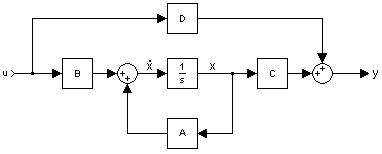
\includegraphics[width=250]{ssm.png}
\caption{\label{fig:ssm.png}SSM Block Diagram}
\end{figure}
\end{frame}

\begin{frame}{State Space Analysis}
    \begin{itemize}
        \item Transfer Function from State Space model: $TF: H(s) = C[sI-A]^{-1}B + D = C\frac{Adj[sI-A]}{|sI-A|}B + D$
        \item $H(s) = \frac{\begin{bmatrix}
        1 & 0
        \end{bmatrix}\begin{bmatrix}
        s+3 & 1\\
        -2 & s
        \end{bmatrix}\begin{bmatrix}
        0\\
        1
        \end{bmatrix}}{s(s+3) + 2} = \LARGE{\frac{1}{s^{2}+3s+2}}$
        \item Therefore the poles of the transfer function are: s = -1 and s = -2
    \end{itemize}
\end{frame}



\begin{frame}{Solution 2}
\begin{block}


\begin{itemize}
\item From first equation: $$\frac{\partial x_1(t)}{\partial t} =              x_2(t) $$
\item Substitution in second equation results into the equation:\vspace{5} $\frac{\partial^2 x_1}{\partial t^2} + 3\frac{\partial x_1(t)}{\partial t} + 2x_1(t) = r(t)$ 
\item Taking Laplace transform on both sides:\vspace{5}
$s^2X_1(s) + 3sX_1(s) + 2X_1(s) - sx_1(0) - x_1'(0) -3x_1(0)  = R(s)$
\item $ H(s) = \frac{X_1(s)}{R(s)} = \frac{1}{s^2 + 3s + 2}$
\item Therefore the poles of the transfer function are: s = -1 and s = -2
\end{itemize}
\end{block}

\end{frame}

\subsection{Result}

\begin{frame}{Result and Conclusion}

\begin{itemize}
    \item Since the poles of the transfer function are real and distinct, the system is \textbf{OVERDAMPED}.
    \item Solution: $h(t) = L^{-1}(H(s)) = e^{-t} - e^{-2t}$
\end{itemize}

\end{frame}

\end{document}
